% !TEX program = xelatex
\documentclass[11pt,a4paper]{article}
\usepackage[margin=2cm,top=1.8cm,bottom=1.8cm]{geometry}
\usepackage{fontspec}
\usepackage{amsmath,amssymb}
\usepackage{graphicx}
\usepackage{enumitem}
\usepackage{booktabs}
\usepackage{array}
\usepackage{tikz}
\usetikzlibrary{arrows.meta,calc}
\usepackage[hidelinks]{hyperref}
\usepackage{fancyhdr}

\pagestyle{fancy}
\fancyhf{}
\lhead{\small Discrete Mathematics --- Previous Year Questions}
\rhead{\small SEC, Sylhet \,|\, CSE 1-1}
\cfoot{\small\thepage}
\renewcommand{\headrulewidth}{0.3pt}
\setlength{\parindent}{0pt}
\setlength{\parskip}{3pt}

\tikzset{
  >={Stealth[length=2mm,width=1.6mm]},
  v/.style={circle,draw,minimum size=5.5mm,inner sep=0pt,font=\footnotesize},
  d/.style={circle,fill,inner sep=1.3pt},
  wt/.style={midway,fill=white,inner sep=1pt,font=\scriptsize},
  every picture/.style={line width=0.5pt},
}

\newcommand{\mk}[1]{\hfill\textbf{[#1]}}
\newcommand{\srcnote}[1]{{\footnotesize\itshape Source: #1}\par\smallskip}
\renewcommand{\partname}[2]{\begin{center}\textbf{\underline{#1}}\\[-1pt]{\small #2}\end{center}}
\newcommand{\OR}{\begin{center}\textbf{OR}\end{center}\vspace{-6pt}}
\newenvironment{Ql}{\begin{enumerate}[leftmargin=2.5em,labelsep=0.4em,itemsep=5pt,topsep=2pt]}{\end{enumerate}}
\newenvironment{Sl}{\begin{enumerate}[leftmargin=2.3em,labelsep=0.3em,itemsep=3pt,topsep=2pt]}{\end{enumerate}}
\newenvironment{Rl}{\begin{enumerate}[leftmargin=2.2em,labelsep=0.3em,itemsep=1pt,topsep=1pt]}{\end{enumerate}}
\newcommand{\scanfig}[1]{\par\medskip\begin{center}#1\end{center}\par}

\newcommand{\paperhead}[5]{%
\begin{center}
{\large\bfseries Sylhet Engineering College, Sylhet}\\
{\small (Shahjalal University of Science \& Technology)}\\
{\small Department of Computer Science \& Engineering}
\end{center}
\vspace{-2pt}
\noindent\begin{tabular*}{\linewidth}{@{}l@{\extracolsep{\fill}}r@{}}
\textbf{#1} & 1\textsuperscript{st} Year 1\textsuperscript{st} Semester\\
\textbf{Course No:} #2 & \textbf{Course Title:} #5\\
\textbf{Time:} #3 & \textbf{Full Marks:} #4
\end{tabular*}\par\smallskip\hrule\medskip}

%%%%%%%%%%%%%%%%%%%%%%%%% FIGURES %%%%%%%%%%%%%%%%%%%%%%%%%

% fan graph (spanning-tree questions)
\newcommand{\FigFan}{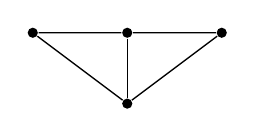
\begin{tikzpicture}
\node[d] (a) at (-1.2,0.9){}; \node[d] (b) at (0,0.9){}; \node[d] (c) at (1.2,0.9){}; \node[d] (e) at (0,0){};
\draw (a)--(b)--(c)--(e)--(a); \draw (b)--(e);
\end{tikzpicture}}

% incidence-matrix graph
\newcommand{\FigInc}{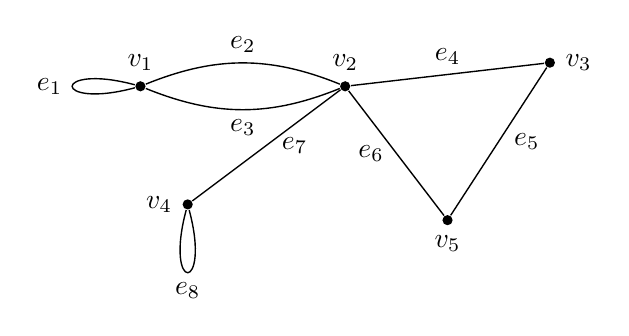
\begin{tikzpicture}[scale=1]
\node[d,label=above:{$v_1$}] (v1) at (0,0){};
\node[d,label=above:{$v_2$}] (v2) at (2.6,0){};
\node[d,label=right:{$v_3$}] (v3) at (5.2,0.3){};
\node[d,label=below:{$v_5$}] (v5) at (3.9,-1.7){};
\node[d,label=left:{$v_4$}] (v4) at (0.6,-1.5){};
\draw (v1) to[loop left,min distance=11mm] node[left]{$e_1$} (v1);
\draw (v1) to[bend left=22] node[above]{$e_2$} (v2);
\draw (v1) to[bend right=22] node[below]{$e_3$} (v2);
\draw (v2) -- node[above]{$e_4$} (v3);
\draw (v3) -- node[right,xshift=2pt]{$e_5$} (v5);
\draw (v2) -- node[left,xshift=-1pt]{$e_6$} (v5);
\draw (v2) -- node[right,xshift=2pt]{$e_7$} (v4);
\draw (v4) to[loop below,min distance=11mm] node[below]{$e_8$} (v4);
\end{tikzpicture}}

% functions f,g,h diagram
\newcommand{\FigFunc}{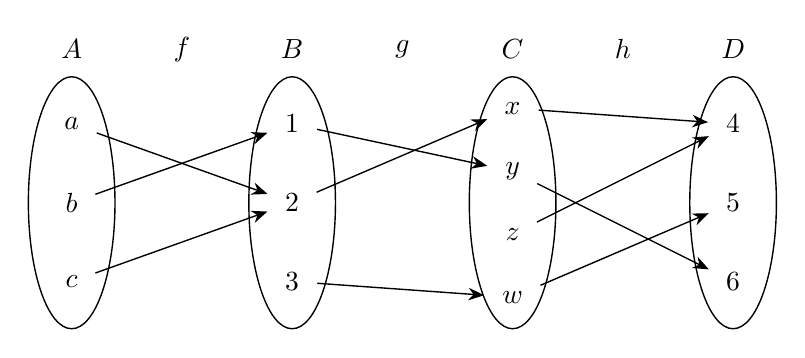
\begin{tikzpicture}
\foreach \x/\l in {0/A,2.8/B,5.6/C,8.4/D}{\draw (\x,0) ellipse (0.55 and 1.6); \node at (\x,1.95){$\l$};}
\node at (1.4,1.95){$f$}; \node at (4.2,1.95){$g$}; \node at (7.0,1.95){$h$};
\node (Aa) at (0,1){$a$}; \node (Ab) at (0,0){$b$}; \node (Ac) at (0,-1){$c$};
\node (B1) at (2.8,1){$1$}; \node (B2) at (2.8,0){$2$}; \node (B3) at (2.8,-1){$3$};
\node (Cx) at (5.6,1.2){$x$}; \node (Cy) at (5.6,0.4){$y$}; \node (Cz) at (5.6,-0.4){$z$}; \node (Cw) at (5.6,-1.2){$w$};
\node (D4) at (8.4,1){$4$}; \node (D5) at (8.4,0){$5$}; \node (D6) at (8.4,-1){$6$};
\begin{scope}[->,shorten >=3pt,shorten <=3pt]
\draw (Aa)--(B2); \draw (Ab)--(B1); \draw (Ac)--(B2);
\draw (B1)--(Cy); \draw (B2)--(Cx); \draw (B3)--(Cw);
\draw (Cx)--(D4); \draw (Cy)--(D6); \draw (Cz)--(D4); \draw (Cw)--(D5);
\end{scope}
\end{tikzpicture}}

% Kruskal graph (CSE-15 Fig.-3)
\newcommand{\FigKruskal}{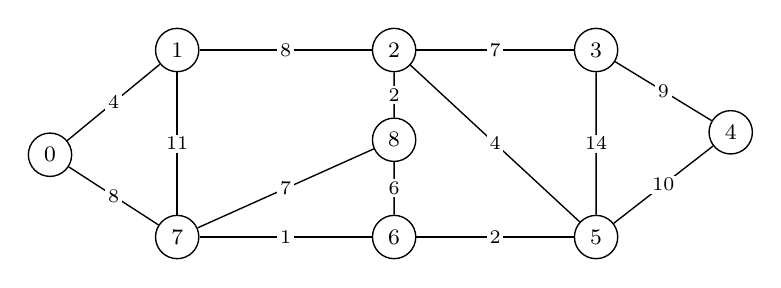
\begin{tikzpicture}[scale=0.95]
\node[v] (n0) at (0,0.2){0}; \node[v] (n1) at (1.7,1.6){1}; \node[v] (n2) at (4.6,1.6){2};
\node[v] (n3) at (7.3,1.6){3}; \node[v] (n4) at (9.1,0.5){4}; \node[v] (n5) at (7.3,-0.9){5};
\node[v] (n6) at (4.6,-0.9){6}; \node[v] (n7) at (1.7,-0.9){7}; \node[v] (n8) at (4.6,0.4){8};
\draw (n0)--node[wt]{4}(n1); \draw (n0)--node[wt]{8}(n7); \draw (n1)--node[wt]{8}(n2);
\draw (n1)--node[wt]{11}(n7); \draw (n2)--node[wt]{7}(n3); \draw (n2)--node[wt]{2}(n8);
\draw (n2)--node[wt]{4}(n5); \draw (n3)--node[wt]{9}(n4); \draw (n3)--node[wt]{14}(n5);
\draw (n4)--node[wt]{10}(n5); \draw (n5)--node[wt]{2}(n6); \draw (n6)--node[wt]{1}(n7);
\draw (n6)--node[wt]{6}(n8); \draw (n7)--node[wt]{7}(n8);
\end{tikzpicture}}

% DFS digraph (CSE-15)
\newcommand{\FigDFS}{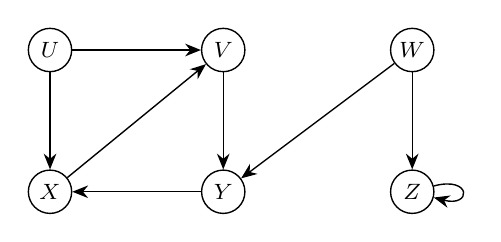
\begin{tikzpicture}
\node[v] (U) at (0,1.8){$U$}; \node[v] (V) at (2.2,1.8){$V$}; \node[v] (W) at (4.6,1.8){$W$};
\node[v] (X) at (0,0){$X$}; \node[v] (Y) at (2.2,0){$Y$}; \node[v] (Z) at (4.6,0){$Z$};
\draw[->] (U)--(V); \draw[->] (U)--(X); \draw[->] (X)--(V); \draw[->] (V)--(Y);
\draw[->] (W)--(Y); \draw[->] (Y)--(X); \draw[->] (W)--(Z); \draw[->] (Z) to[loop right] (Z);
\end{tikzpicture}}

% binary search tree (CSE-15)
\newcommand{\FigBST}{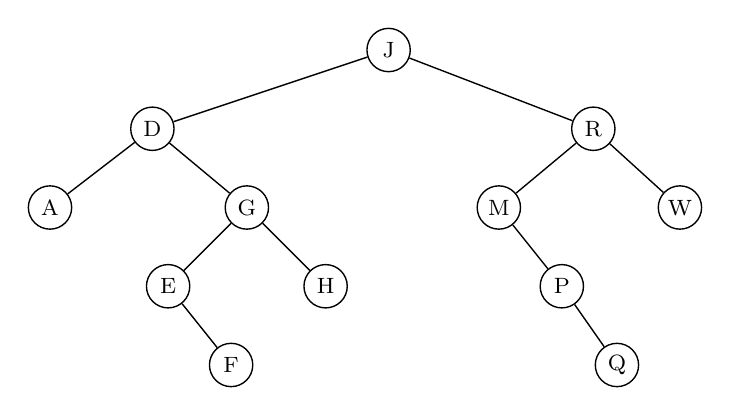
\begin{tikzpicture}[level distance=8mm]
\node[v] (J) at (0,0){J}; \node[v] (D) at (-3,-1){D}; \node[v] (R) at (2.6,-1){R};
\node[v] (A) at (-4.3,-2){A}; \node[v] (G) at (-1.8,-2){G}; \node[v] (E) at (-2.8,-3){E};
\node[v] (H) at (-0.8,-3){H}; \node[v] (F) at (-2.0,-4){F}; \node[v] (M) at (1.4,-2){M};
\node[v] (W) at (3.7,-2){W}; \node[v] (P) at (2.2,-3){P}; \node[v] (Q) at (2.9,-4){Q};
\draw (J)--(D); \draw (J)--(R); \draw (D)--(A); \draw (D)--(G); \draw (G)--(E); \draw (G)--(H);
\draw (E)--(F); \draw (R)--(M); \draw (R)--(W); \draw (M)--(P); \draw (P)--(Q);
\end{tikzpicture}}

% CSE-15 TT2 weighted grid graph
\newcommand{\FigGrid}{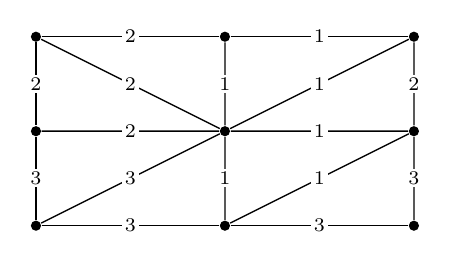
\begin{tikzpicture}[scale=1.2]
\foreach \n/\x/\y in {TL/0/2,TM/2/2,TR/4/2,ML/0/1,C/2/1,MR/4/1,BL/0/0,BM/2/0,BR/4/0}{\node[d] (\n) at (\x,\y){};}
\draw (TL)--node[wt]{2}(TM); \draw (TM)--node[wt]{1}(TR); \draw (TL)--node[wt]{2}(ML);
\draw (TL)--node[wt]{2}(C); \draw (TM)--node[wt]{1}(C); \draw (C)--node[wt]{1}(TR);
\draw (ML)--node[wt]{2}(C); \draw (C)--node[wt]{1}(MR); \draw (TR)--node[wt]{2}(MR);
\draw (ML)--node[wt]{3}(BL); \draw (BL)--node[wt]{3}(C); \draw (C)--node[wt]{1}(BM);
\draw (BM)--node[wt]{1}(MR); \draw (MR)--node[wt]{3}(BR); \draw (BL)--node[wt]{3}(BM);
\draw (BM)--node[wt]{3}(BR);
\end{tikzpicture}}

% Prim graph a..g
\newcommand{\FigPrimG}{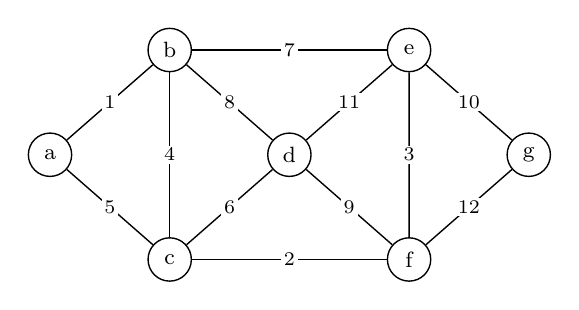
\begin{tikzpicture}[scale=0.95]
\node[v] (a) at (0,0){a}; \node[v] (b) at (1.6,1.4){b}; \node[v] (e) at (4.8,1.4){e};
\node[v] (c) at (1.6,-1.4){c}; \node[v] (f) at (4.8,-1.4){f}; \node[v] (d) at (3.2,0){d};
\node[v] (g) at (6.4,0){g};
\draw (a)--node[wt]{1}(b); \draw (a)--node[wt]{5}(c); \draw (b)--node[wt]{4}(c);
\draw (b)--node[wt]{8}(d); \draw (b)--node[wt]{7}(e); \draw (c)--node[wt]{6}(d);
\draw (c)--node[wt]{2}(f); \draw (d)--node[wt]{11}(e); \draw (d)--node[wt]{9}(f);
\draw (e)--node[wt]{3}(f); \draw (e)--node[wt]{10}(g); \draw (f)--node[wt]{12}(g);
\end{tikzpicture}}

% Dijkstra graph 0..6 (CSE-17 TT2)
\newcommand{\FigDijZero}{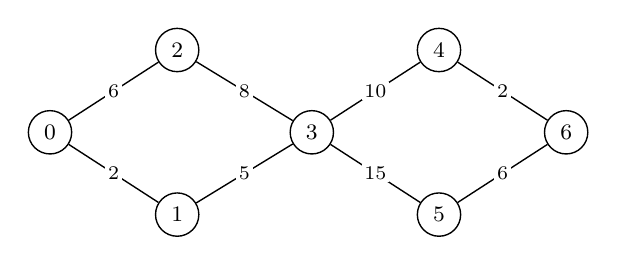
\begin{tikzpicture}[scale=0.95]
\node[v] (n0) at (0,0){0}; \node[v] (n2) at (1.7,1.1){2}; \node[v] (n1) at (1.7,-1.1){1};
\node[v] (n3) at (3.5,0){3}; \node[v] (n4) at (5.2,1.1){4}; \node[v] (n5) at (5.2,-1.1){5};
\node[v] (n6) at (6.9,0){6};
\draw (n0)--node[wt]{6}(n2); \draw (n0)--node[wt]{2}(n1); \draw (n2)--node[wt]{8}(n3);
\draw (n1)--node[wt]{5}(n3); \draw (n3)--node[wt]{10}(n4); \draw (n3)--node[wt]{15}(n5);
\draw (n4)--node[wt]{2}(n6); \draw (n5)--node[wt]{6}(n6);
\end{tikzpicture}}

% BFS graph (CSE-17 final)
\newcommand{\FigBFS}{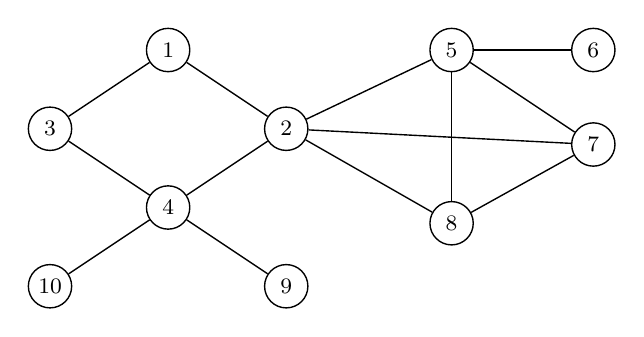
\begin{tikzpicture}
\node[v] (n1) at (0,2.4){1}; \node[v] (n3) at (-1.5,1.4){3}; \node[v] (n2) at (1.5,1.4){2};
\node[v] (n4) at (0,0.4){4}; \node[v] (n10) at (-1.5,-0.6){10}; \node[v] (n9) at (1.5,-0.6){9};
\node[v] (n5) at (3.6,2.4){5}; \node[v] (n6) at (5.4,2.4){6}; \node[v] (n7) at (5.4,1.2){7};
\node[v] (n8) at (3.6,0.2){8};
\draw (n1)--(n3); \draw (n1)--(n2); \draw (n3)--(n4); \draw (n2)--(n4); \draw (n4)--(n10);
\draw (n4)--(n9); \draw (n2)--(n5); \draw (n2)--(n7); \draw (n2)--(n8); \draw (n5)--(n6);
\draw (n5)--(n7); \draw (n5)--(n8); \draw (n7)--(n8);
\end{tikzpicture}}

% Floyd--Warshall digraph
\newcommand{\FigFloyd}{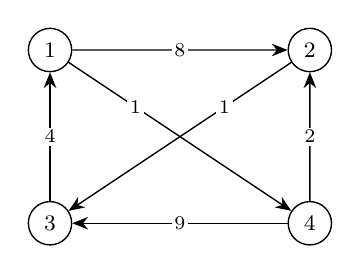
\begin{tikzpicture}[scale=1.1]
\node[v] (n1) at (0,2){1}; \node[v] (n2) at (3,2){2}; \node[v] (n3) at (0,0){3}; \node[v] (n4) at (3,0){4};
\draw[->] (n1)--node[wt]{8}(n2); \draw[->] (n3)--node[wt]{4}(n1); \draw[->] (n4)--node[wt]{2}(n2);
\draw[->] (n4)--node[wt]{9}(n3); \draw[->] (n1)--node[wt,pos=0.3]{1}(n4); \draw[->] (n2)--node[wt,pos=0.3]{1}(n3);
\end{tikzpicture}}

% CSE-16 Fig-1 digraph
\newcommand{\FigSixteenOne}{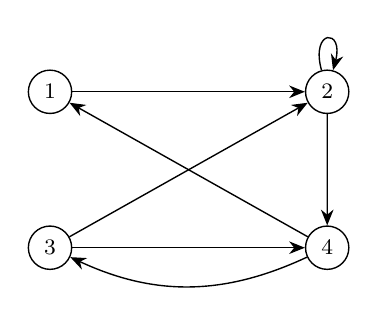
\begin{tikzpicture}[scale=1.1]
\node[v] (n1) at (0,1.8){1}; \node[v] (n2) at (3.2,1.8){2}; \node[v] (n3) at (0,0){3}; \node[v] (n4) at (3.2,0){4};
\draw[->] (n1)--(n2); \draw[->] (n2) to[loop above] (n2); \draw[->] (n2)--(n4);
\draw[->] (n3)--(n2); \draw[->] (n3)--(n4); \draw[->] (n4)--(n1);
\draw[->] (n4) to[bend left=25] (n3);
\end{tikzpicture}}

% CSE-16 Fig-2 (DFS)
\newcommand{\FigSixteenTwo}{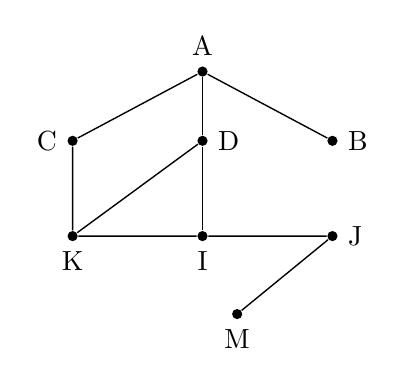
\begin{tikzpicture}[scale=1.1]
\node[d,label=above:A] (A) at (0,2.6){}; \node[d,label=left:C] (C) at (-1.5,1.8){};
\node[d,label=right:D] (D) at (0,1.8){}; \node[d,label=right:B] (B) at (1.5,1.8){};
\node[d,label=below:K] (K) at (-1.5,0.7){}; \node[d,label=below:I] (I) at (0,0.7){};
\node[d,label=right:J] (J) at (1.5,0.7){}; \node[d,label=below:M] (M) at (0.4,-0.2){};
\draw (A)--(C); \draw (A)--(D); \draw (A)--(B); \draw (C)--(K); \draw (D)--(K); \draw (D)--(I);
\draw (K)--(I); \draw (I)--(J); \draw (J)--(M);
\end{tikzpicture}}

% CSE-16 Fig-3 (articulation)
\newcommand{\FigSixteenThree}{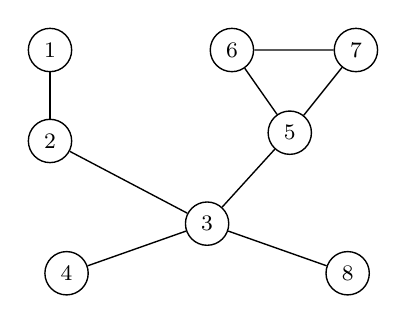
\begin{tikzpicture}[scale=1.05]
\node[v] (n1) at (0,2.7){1}; \node[v] (n2) at (0,1.6){2}; \node[v] (n3) at (1.9,0.6){3};
\node[v] (n4) at (0.2,0){4}; \node[v] (n8) at (3.6,0){8}; \node[v] (n5) at (2.9,1.7){5};
\node[v] (n6) at (2.2,2.7){6}; \node[v] (n7) at (3.7,2.7){7};
\draw (n1)--(n2); \draw (n2)--(n3); \draw (n3)--(n4); \draw (n3)--(n8); \draw (n3)--(n5);
\draw (n5)--(n6); \draw (n5)--(n7); \draw (n6)--(n7);
\end{tikzpicture}}

% CSE-16 Fig-4 digraph
\newcommand{\FigSixteenFour}{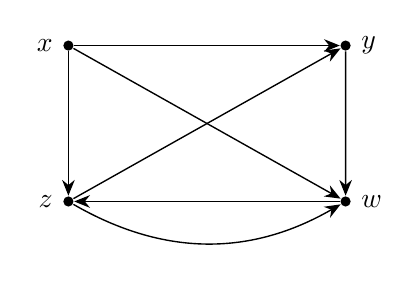
\begin{tikzpicture}[scale=1.1]
\node[d,label=left:$x$] (x) at (0,1.8){}; \node[d,label=right:$y$] (y) at (3.2,1.8){};
\node[d,label=left:$z$] (z) at (0,0){}; \node[d,label=right:$w$] (w) at (3.2,0){};
\draw[->] (x)--(y); \draw[->] (x)--(z); \draw[->] (x)--(w); \draw[->] (z)--(y);
\draw[->] (y)--(w); \draw[->] (w)--(z); \draw[->] (z) to[bend right=30] (w);
\end{tikzpicture}}

% heptagon / heptagram pair
\newcommand{\FigIso}{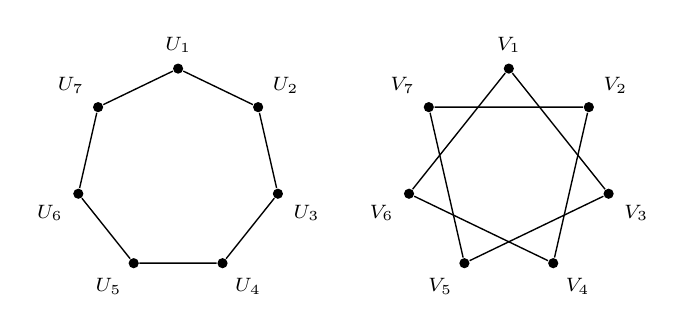
\begin{tikzpicture}[scale=1.0]
\foreach \i in {1,...,7}{%
 \pgfmathsetmacro{\a}{90-360/7*(\i-1)}
 \node[d,label={[font=\scriptsize]\a:$U_\i$}] (u\i) at (\a:1.3){};
 \node[d,label={[font=\scriptsize]\a:$V_\i$}] (w\i) at ([shift={(4.2,0)}]\a:1.3){};}
\foreach \i in {1,...,7}{%
 \pgfmathtruncatemacro{\j}{mod(\i,7)+1}
 \pgfmathtruncatemacro{\k}{mod(\i+1,7)+1}
 \draw (u\i)--(u\j); \draw (w\i)--(w\k);}
\end{tikzpicture}}

% CSE-16 Dijkstra digraph
\newcommand{\FigSixteenDij}{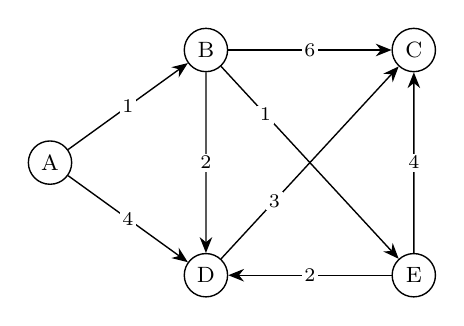
\begin{tikzpicture}[scale=1.1]
\node[v] (A) at (0,0){A}; \node[v] (B) at (1.8,1.3){B}; \node[v] (C) at (4.2,1.3){C};
\node[v] (D) at (1.8,-1.3){D}; \node[v] (E) at (4.2,-1.3){E};
\draw[->] (A)--node[wt]{1}(B); \draw[->] (A)--node[wt]{4}(D); \draw[->] (B)--node[wt]{6}(C);
\draw[->] (B)--node[wt]{2}(D); \draw[->] (B)--node[wt,pos=0.25]{1}(E); \draw[->] (D)--node[wt,pos=0.3]{3}(C);
\draw[->] (E)--node[wt]{4}(C); \draw[->] (E)--node[wt]{2}(D);
\end{tikzpicture}}

% planar graph question
\newcommand{\FigPlanar}{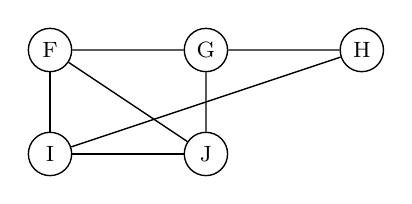
\begin{tikzpicture}[scale=1.1]
\node[v] (F) at (0,1.2){F}; \node[v] (G) at (1.8,1.2){G}; \node[v] (H) at (3.6,1.2){H};
\node[v] (I) at (0,0){I}; \node[v] (J) at (1.8,0){J};
\draw (F)--(G)--(H); \draw (F)--(I); \draw (F)--(J); \draw (G)--(J); \draw (H)--(I); \draw (I)--(J);
\end{tikzpicture}}

% connected-graph pair
\newcommand{\FigConn}{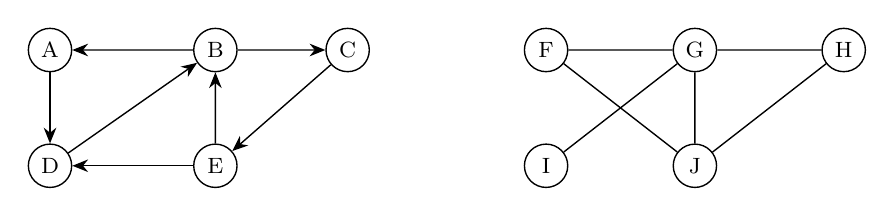
\begin{tikzpicture}[scale=1.05]
\node[v] (A) at (0,1.4){A}; \node[v] (B) at (2,1.4){B}; \node[v] (C) at (3.6,1.4){C};
\node[v] (D) at (0,0){D}; \node[v] (E) at (2,0){E};
\draw[->] (B)--(A); \draw[->] (B)--(C); \draw[->] (A)--(D); \draw[->] (D)--(B);
\draw[->] (E)--(B); \draw[->] (E)--(D); \draw[->] (C)--(E);
\begin{scope}[xshift=6cm]
\node[v] (F) at (0,1.4){F}; \node[v] (G) at (1.8,1.4){G}; \node[v] (H) at (3.6,1.4){H};
\node[v] (I) at (0,0){I}; \node[v] (J) at (1.8,0){J};
\draw (F)--(G)--(H); \draw (F)--(J); \draw (I)--(G); \draw (G)--(J); \draw (H)--(J);
\end{scope}
\end{tikzpicture}}

% bipartite check graph
\newcommand{\FigBip}{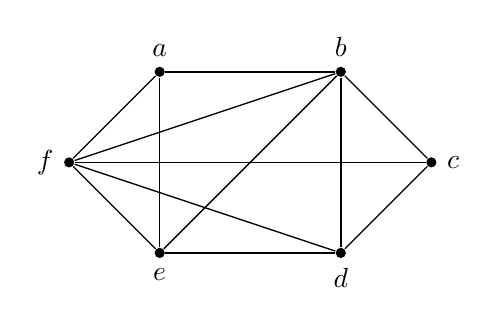
\begin{tikzpicture}[scale=1.15]
\node[d,label=left:$f$] (f) at (-2,0){}; \node[d,label=above:$a$] (a) at (-1,1){};
\node[d,label=above:$b$] (b) at (1,1){}; \node[d,label=right:$c$] (c) at (2,0){};
\node[d,label=below:$e$] (e) at (-1,-1){}; \node[d,label=below:$d$] (d) at (1,-1){};
\draw (a)--(b); \draw (a)--(f); \draw (a)--(e); \draw (b)--(f); \draw (b)--(e); \draw (b)--(c);
\draw (b)--(d); \draw (f)--(c); \draw (f)--(d); \draw (f)--(e); \draw (e)--(d); \draw (c)--(d);
\end{tikzpicture}}

% binary tree A..J
\newcommand{\FigBinTree}{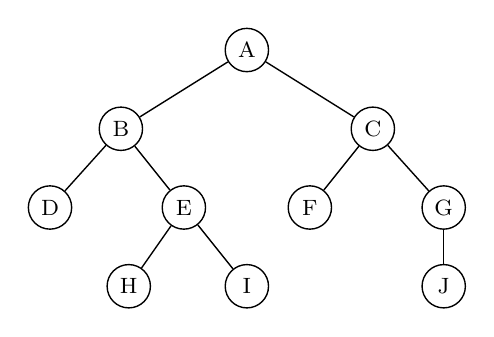
\begin{tikzpicture}[scale=1.0]
\node[v] (A) at (0,0){A}; \node[v] (B) at (-1.6,-1){B}; \node[v] (C) at (1.6,-1){C};
\node[v] (D) at (-2.5,-2){D}; \node[v] (E) at (-0.8,-2){E}; \node[v] (F) at (0.8,-2){F};
\node[v] (G) at (2.5,-2){G}; \node[v] (H) at (-1.5,-3){H}; \node[v] (I) at (0,-3){I};
\node[v] (J) at (2.5,-3){J};
\draw (A)--(B); \draw (A)--(C); \draw (B)--(D); \draw (B)--(E); \draw (C)--(F); \draw (C)--(G);
\draw (E)--(H); \draw (E)--(I); \draw (G)--(J);
\end{tikzpicture}}

% CSE-16 Prim graph
\newcommand{\FigSixteenPrim}{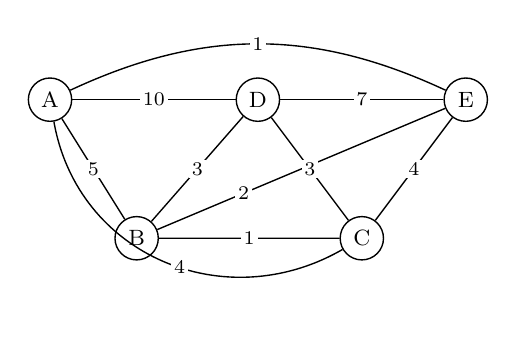
\begin{tikzpicture}[scale=1.1]
\node[v] (A) at (0,0){A}; \node[v] (D) at (2.4,0){D}; \node[v] (E) at (4.8,0){E};
\node[v] (B) at (1,-1.6){B}; \node[v] (C) at (3.6,-1.6){C};
\draw (A) to[bend left=25] node[wt]{1} (E);
\draw (A)--node[wt]{10}(D); \draw (D)--node[wt]{7}(E); \draw (A)--node[wt]{5}(B);
\draw (B)--node[wt]{3}(D); \draw (B)--node[wt,pos=0.3]{2}(E); \draw (D)--node[wt]{3}(C);
\draw (C)--node[wt]{4}(E); \draw (B)--node[wt]{1}(C);
\draw (A) to[out=-80,in=-150,looseness=1.1] node[wt,pos=0.55]{4} (C);
\end{tikzpicture}}

% CSE-16 TT2: strongly / weakly connected pair
\newcommand{\FigStrong}{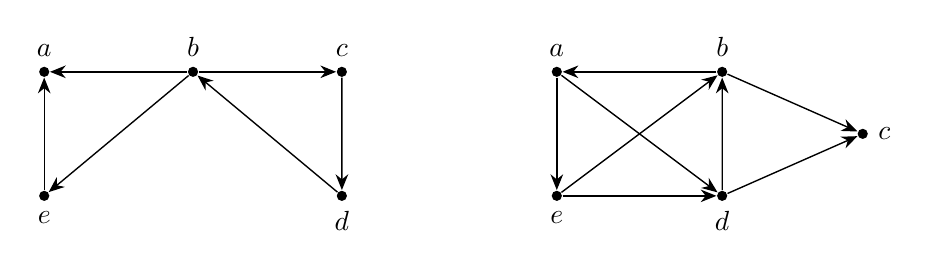
\begin{tikzpicture}[scale=1.05]
\node[d,label=above:$a$] (a) at (0,1.5){}; \node[d,label=above:$b$] (b) at (1.8,1.5){};
\node[d,label=above:$c$] (c) at (3.6,1.5){}; \node[d,label=below:$e$] (e) at (0,0){};
\node[d,label=below:$d$] (d) at (3.6,0){};
\draw[->] (b)--(a); \draw[->] (b)--(c); \draw[->] (e)--(a); \draw[->] (b)--(e);
\draw[->] (d)--(b); \draw[->] (c)--(d);
\begin{scope}[xshift=6.2cm]
\node[d,label=above:$a$] (a) at (0,1.5){}; \node[d,label=above:$b$] (b) at (2,1.5){};
\node[d,label=right:$c$] (c) at (3.7,0.75){}; \node[d,label=below:$e$] (e) at (0,0){};
\node[d,label=below:$d$] (d) at (2,0){};
\draw[->] (b)--(a); \draw[->] (a)--(e); \draw[->] (a)--(d); \draw[->] (e)--(b);
\draw[->] (e)--(d); \draw[->] (d)--(b); \draw[->] (b)--(c); \draw[->] (d)--(c);
\end{scope}
\end{tikzpicture}}

% CSE-16 TT2 Dijkstra (undirected)
\newcommand{\FigTTDij}{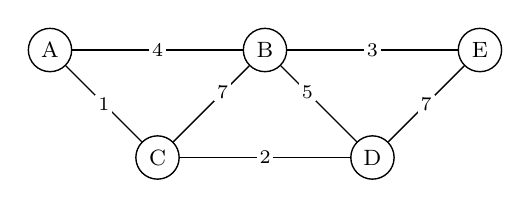
\begin{tikzpicture}[scale=1.05]
\node[v] (A) at (0,0){A}; \node[v] (B) at (2.6,0){B}; \node[v] (E) at (5.2,0){E};
\node[v] (C) at (1.3,-1.3){C}; \node[v] (D) at (3.9,-1.3){D};
\draw (A)--node[wt]{4}(B); \draw (B)--node[wt]{3}(E); \draw (A)--node[wt]{1}(C);
\draw (B)--node[wt,pos=0.35]{7}(C); \draw (B)--node[wt,pos=0.35]{5}(D); \draw (C)--node[wt]{2}(D);
\draw (D)--node[wt]{7}(E);
\end{tikzpicture}}

%%%%%%%%%%%%%%%%%%%%%%%%% DOCUMENT %%%%%%%%%%%%%%%%%%%%%%%%%
\begin{document}

\begin{center}
{\LARGE\bfseries Discrete Mathematics}\\[4pt]
{\Large Previous Year Questions --- CSE 1st Year 1st Semester}\\[4pt]
{\large Sylhet Engineering College, Sylhet}\\[10pt]
{\small Recreated from scanned papers (CSE-15, CSE-16, CSE-17, CSE-18 batches)}
\end{center}
\vspace{6pt}

\tableofcontents

\section{Topic map}
Which topics were asked in which paper.
\textbf{F} = Semester Final, \textbf{TT} = Term Test; the number is the batch (15--18).
\medskip

\newcommand{\B}{$\bullet$}
\begin{center}
\small
\renewcommand{\arraystretch}{1.25}
\begin{tabular}{@{}p{5.0cm}*{11}{>{\centering\arraybackslash}p{0.72cm}}@{}}
\toprule
Topic & \rotatebox{90}{15 F} & \rotatebox{90}{15 TT1} & \rotatebox{90}{15 TT2} & \rotatebox{90}{16 F} & \rotatebox{90}{16 TT2} & \rotatebox{90}{17 TT1} & \rotatebox{90}{17 TT2} & \rotatebox{90}{17 F} & \rotatebox{90}{18 TT1} & \rotatebox{90}{18 TT2} & \rotatebox{90}{18 F}\\
\midrule
Propositional logic, tautology, equivalences &&&&\B&&&&\B&&&\B\\
Rules of inference &&&&&&&&&\B&&\B\\
Sets, Venn diagrams, counting &\B&\B&&&&\B&&\B&&\B&\B\\
Functions, floor/ceiling, composition &\B&\B&&\B&\B&&&\B&&\B&\B\\
Ackermann, recursive definitions &\B&&&\B&&\B&&\B&&\B&\B\\
Relations (properties, matrices, digraphs) &&&&\B&\B&&&&\B&&\B\\
Induction, recurrence relations &&&&\B&&&&&&\B&\B\\
Graph basics (matrices, isomorphism, planar, connected, colouring) &\B&&&\B&\B&&&\B&&&\B\\
Graph traversal (BFS, DFS, articulation point) &\B&&&\B&&&&\B&&&\\
Shortest paths (Dijkstra, Floyd--Warshall) &\B&&&\B&\B&&\B&\B&&&\\
Spanning trees (Prim, Kruskal) &\B&&\B&\B&&&\B&\B&&&\B\\
Trees (binary, BST, traversals, Huffman, 2-trees) &\B&&\B&\B&&&\B&\B&&&\\
Boolean algebra, K-map, logic circuits &&&&&&&&\B&&&\\
Algorithms \& data structures (stack, queue, sorting, searching, Euclid) &&&\B&&&&&\B&&&\\
Permutations &&&&&&&&\B&&&\\
\bottomrule
\end{tabular}
\end{center}

\bigskip
\textbf{Papers found in the scans}

\begin{center}
\small
\begin{tabular}{@{}lll@{}}
\toprule
Batch & Papers & Scan file\\
\midrule
CSE-15 & Final 2022, Term Test 1, Term Test 2 & \texttt{CSE-15\_batch\_all\_question\_\ldots}\\
CSE-16 & Final 2023, Term Test 2 (no TT1 in the scan) & \texttt{[1-1] Semester Final TT 16th batch}\\
CSE-17 & Term Test 1, Term Test 2, Final & \texttt{CSE-17\_(semester final and term test)}\\
CSE-18 & Term Test 1, Term Test 2, Final 2024 & \texttt{CSE-18 [1-1] TT \& Semester Questions}\\
CSE-18 & Final 2024 (same paper as above) & \texttt{2024-25 CSE semster final 1-1}\\
\bottomrule
\end{tabular}
\end{center}

%%%%%%%%%%%%%%%%%%%%%%%%%%%%%%%%%%%%%%%%%%%%%%%%%%%%%%%%%%%
\clearpage
\section{CSE-15 batch}
\subsection{Final Examination, 2022}
\srcnote{CSE-15 batch file, Discrete Mathematics final (2 pages).}
\paperhead{Final Examination, 2022}{CSE 103}{02 (Two) hours}{40}{Discrete Mathematics}
{\small N.B.: (i) Answer any two question from each PART \quad (ii) Use separate answer scripts for each PART \quad (iii) Marks allotted are indicated in the margin \quad (iv) Special Instruction (if any): N/A}

\partname{PART-A}{(Answer any two question)}
\begin{Ql}
\item[\textbf{1)}]
 \begin{Sl}
 \item[a)] Which of these sets are equal: $\{x,y,z\}$, $\{z,y,z,x\}$, $\{y,x,y,z\}$, $\{y,z,x,y\}$? \mk{2}
 \item[b)] List the elements of each set where $\mathbb N=\{1,2,3,\dots\}$. \mk{$1\times3$}
  \begin{Rl}
  \item[(i)] $A=\{x\in\mathbb N \mid 3<x<9\}$
  \item[(ii)] $B=\{x\in\mathbb N \mid x \text{ is even},\ x<11\}$
  \item[(iii)] $C=\{x\in\mathbb N \mid 4+x=3\}$
  \end{Rl}
 \item[c)] Determine which of the following sets are finite: \mk{2}
  \begin{Rl}
  \item[(i)] Lines parallel to the $x$ axis.
  \item[(ii)] Letters in the English alphabet.
  \item[(iii)] Integers which are multiples of 5.
  \item[(iv)] Animals living on the earth.
  \end{Rl}
 \item[d)] Each student in Liberal Arts at some college has a mathematics requirement $A$ and a science requirement $B$. A poll of 140 sophomore students shows that: 60 completed $A$, 45 completed $B$, 20 completed both $A$ and $B$. Use a Venn diagram to find the number of students who have completed: (i) At least one of $A$ and $B$; (ii) exactly one of $A$ or $B$; (iii) neither $A$ nor $B$. \mk{$1\times3$}
 \end{Sl}
\item[\textbf{2)}]
 \begin{Sl}
 \item[(a)] Adjacency matrix of the directed graph $G$ with vertices $X,Y,Z,W$ is given below: \mk{6}
  \[A=\begin{pmatrix}0&0&0&1\\1&0&1&1\\1&0&0&1\\1&0&1&0\end{pmatrix}\]
  i) Draw the directed graph $G$.\quad ii) Find the powers $A^2$.
 \item[(b)] Plot the following functions: (i) $\left\lceil \dfrac{x}{2}\right\rceil$ \quad (ii) $\left\lfloor \dfrac{x}{2}\right\rfloor$ \mk{4}
 \end{Sl}
\item[\textbf{3)}]
 \begin{Sl}
 \item[a)] Let the functions $f\colon A\to B$, $g\colon B\to C$, $h\colon C\to D$ be defined by Fig.-1. Determine if each function is: (i) onto, (ii) one-to-one, (iii) invertible. \mk{$1\times3$}
  \scanfig{\FigFunc\\[2pt]Figure-1}
 \item[b)] Find the cardinal number of each set: \mk{2}\\
  (i) $A=\{a,b,c,\dots,y,z\}$, \hfill (iii) $C=\{10,20,30,40,\dots\}$,\\
  (ii) $B=\{x\mid x\in\mathbb N,\ x^{2}=5\}$, \hfill (iv) $D=\{6,7,8,9,\dots\}$.
 \item[c)] Find: (a) $\lfloor 7.5\rfloor,\ \lfloor -7.5\rfloor,\ \lfloor -18\rfloor$; (b) $\lceil 7.5\rceil,\ \lceil -7.5\rceil,\ \lceil -18\rceil$. \mk{2}
 \item[d)] \textbf{Ackermann function:} \mk{3}\\
  (a) If $m=0$, then $A(m,n)=n+1$.\\
  (b) If $m\neq0$ but $n=0$, then $A(m,n)=A(m-1,1)$.\\
  (c) If $m\neq0$ and $n\neq0$, then $A(m,n)=A(m-1,A(m,n-1))$.\\
  Use the definition of the Ackermann function to find $A(2,2)$.
 \end{Sl}
\end{Ql}

\partname{PART-B}{(Answer any two question)}
\begin{Ql}
\item[\textbf{4)}]
 \begin{Sl}
 \item[a)] Define the following term with examples. i) sub-graph \quad ii) complete graph \quad iii) Bipartite graph \quad iv) Regular graph. \mk{2}
 \item[b)] Prove that: The sum of the degrees of the regions of a map is equal to twice the number of edges. \mk{2}
 \item[c)] Find all spanning trees of the graph $G$ shown in figure-2. \mk{2}
  \scanfig{\FigFan\\[2pt]Figure:-2}
 \item[d)] Find a minimal cost spanning tree $T$ for the weighted graph $G$ in Fig.-3 using Kruskal's algorithm. \mk{4}
  \scanfig{\FigKruskal\\[2pt]Figure -3}
 \end{Sl}
\item[\textbf{5)}]
 \begin{Sl}
 \item[a)] Define vertex coloring and chromatic number. \mk{2}
 \item[b)] Consider the following weighted graph $G$. Suppose the nodes are stored in an array DATA as follows: DATA: $X,Y,S,T$. Find the matrix $Q$ of shortest paths using Warshall's Algorithm. \mk{4}
  \scanfig{\fbox{\parbox{0.6\linewidth}{\centering\itshape\small [The weighted graph is blacked out in the scan and cannot be recovered.]}}}
 \item[c)] Compute the DFS tree for the graph given below. \mk{4}
  \scanfig{\FigDFS}
 \end{Sl}
\item[\textbf{6)}]
 \begin{Sl}
 \item[i)] From the following binary search tree insert the nodes C, Z and T. \mk{6+4}
  \scanfig{\FigBST}
 \item[ii)] Find the in-order, pre-order and post-order traversal of the above tree shown in figure.
 \end{Sl}
\end{Ql}

%%%%%%%%%%%%%%%%%%%%%%%%%%%%%%%%%%%%%%%%%%%%%%%%%%%%%%%%%%%
\clearpage
\subsection{Term Test-01}
\srcnote{CSE-15 batch file (upper half of the term-test page).}
\begin{center}
{\bfseries Sylhet Engineering College, Sylhet}\\
Department of Computer Science and Engineering\\
1\textsuperscript{st} year 1\textsuperscript{st} Semester \quad Course No: CSE-103 \quad Course Title: Discrete Mathematics\\
Time: 20 min \quad Total Marks: 15
\end{center}
\begin{Ql}
\item Suppose a list $A$ contains the 30 students in a mathematics class, and a list $B$ contains the 35 students in an English class, and suppose there are 20 names on both lists. Find the number of students: (a) only on list $A$, (b) only on list $B$, (c) on list $A$ or $B$ (or both), (d) on exactly one list. \mk{5}
\item Let $A=\{1,2,3\}$, $B=\{a,b,c,d\}$ and $C=\{c,d\}$. Find: $(A\times B)\cap(A\times C)$ and $(B\cap C)$. \mk{5}
\item Find: (a) $\lfloor 7.5\rfloor,\ \lfloor -7.5\rfloor,\ \lfloor -18\rfloor$; (b) $\lceil 7.5\rceil,\ \lceil -7.5\rceil,\ \lceil -18\rceil$. \mk{5}
\end{Ql}

\subsection{Term Test-02}
\srcnote{CSE-15 batch file (lower half of the same page order as scanned).}
\begin{center}
{\bfseries Sylhet Engineering College, Sylhet}\\
Department of Computer Science and Engineering\\
1\textsuperscript{st} year 1\textsuperscript{st} Semester \quad Course No: CSE-103 \quad Course Title: Discrete Mathematics\\
Time: 20 min \quad Total Marks: 15
\end{center}
\begin{Ql}
\item Find a minimal spanning tree $T$ for the weighted graph $G$ in Fig.~(a). \mk{7}
 \scanfig{\FigGrid\\[2pt](a)}
\item Consider the algebraic expression $E=(2x+y)(5a-b)^3$. Draw the corresponding 2-tree. Use an arrow ($\uparrow$) for exponentiation, an asterisk ($*$) for multiplication, and a slash ($/$) for division. \mk{5}
\item Define Stacks, Queues, and Priority Queues. \mk{3}
\end{Ql}

%%%%%%%%%%%%%%%%%%%%%%%%%%%%%%%%%%%%%%%%%%%%%%%%%%%%%%%%%%%
\clearpage
\section{CSE-16 batch}
\subsection{Final Examination, 2023}
\srcnote{CSE-16 batch file (3 pages).}
\paperhead{Final Examination, 2023}{CSE 143}{03 (Three) hours}{60}{Discrete Mathematics}
{\small N.B.: (i) Answer any three questions from each PART \quad (ii) Use separate answer scripts for each PART \quad (iii) Marks allotted are indicated in the margin \quad (iv) Special Instruction (if any): N/A}

\partname{PART-A}{(Answer any three questions)}
\begin{Ql}
\item[\textbf{1.}]
 \begin{Sl}
 \item[(a)] Let $p=$ ``It is raining today'' and $q=$ ``CSE first semester exam will take place.'' Write down the above propositional statements in English: (a) $p\to q$ \ (b) $q\leftrightarrow\neg p$. \mk{2}
 \item[(b)] Determine whether the statement $(\neg p\wedge\neg q)\leftrightarrow(q\to r)$ is a tautology or contradiction or contingency. \mk{5}
 \item[(c)] Show that $(p\to q)\wedge(p\to r)$ and $p\to(q\wedge r)$ are logically equivalent by developing a series of logical equivalences. \mk{3}
 \end{Sl}
\item[\textbf{2.}]
 \begin{Sl}
 \item[(a)] Define Relation. Find the relation determined by the figure-1: \mk{1+2}
  \scanfig{\FigSixteenOne\\[2pt]Figure-1}
 \item[(b)] Given $A=\{1,2,3,4\}$ and $B=\{x,y,z\}$. Let $R$ be the following relation from $A$ to $B$:
  $R=\{(1,y),(1,z),(3,y),(4,x),(4,z)\}$ \mk{4}
  \begin{Rl}
  \item[(i)] Determine the matrix of the relation.
  \item[(ii)] Draw the arrow diagram of $R$.
  \item[(iii)] Find the inverse relation $R^{-1}$ of $R$.
  \item[(iv)] Determine the domain and range of $R$.
  \end{Rl}
 \item[(c)] Consider the relation $R=\{(a,a),(a,b),(b,c),(c,c)\}$ on the set $A=\{a,b,c\}$. Find: (i) reflexive$(R)$; (ii) symmetric$(R)$; (iii) transitive$(R)$. \mk{3}
 \end{Sl}
\item[\textbf{3.}]
 \begin{Sl}
 \item[(a)] Find out value of given expressions.
  \[\left\lfloor\tfrac15\right\rfloor\qquad \lceil 2.5\rceil\qquad \lfloor -2.99\rfloor\qquad \left\lceil-\tfrac12\right\rceil\] \mk{2}
 \item[(b)] If $f(x)=x^2+1$ is a function from $\mathbb R$ to $\mathbb R$. Is it a one-to-one correspondence? \mk{4}
 \item[(c)] Let $f$ and $g$ be the functions from the set of integers to the set of integers defined by $f(x)=2x+3$ and $g(x)=3x^2+2$. Determine $f\circ g(3)$ and $g\circ f(1)$. \mk{4}
 \end{Sl}
\item[\textbf{4.}]
 \begin{Sl}
 \item[(a)] Use mathematical induction to show that
  \[\sum_{p=1}^{n}p^3=\frac{n^2(n+1)^2}{4}\]
  for all nonnegative integers $n$. \mk{5}
 \item[(b)] Suppose that $f$ is defined recursively by $f(0)=0$, $f(1)=1$, $f(n)=f(n-1)+f(n-2)$. Find out the value of $f(7)$. \mk{5}
 \end{Sl}
\end{Ql}

\partname{PART-B}{(Answer any three questions)}
\begin{Ql}
\item[\textbf{5.}]
 \begin{Sl}
 \item[(a)] If on the particular given graph in Fig.~2 if you execute DFS algorithm write the sequence in which nodes are getting traversed: \mk{4}
  \scanfig{\FigSixteenTwo\\[2pt]Fig. 2}
 \item[(b)] Define Articulation Point. Find the articulation point for Fig.~3: \mk{1+3}
  \scanfig{\FigSixteenThree\\[2pt]Fig. 3}
 \item[(c)] Let $G$ be the directed graph in Fig~4. (a) Find the indegree and outdegree of each vertex of $G$. (b) Find the successor list of each vertex of $G$. \mk{1+1}
  \scanfig{\FigSixteenFour\\[2pt]Fig. 4}
 \end{Sl}
\item[\textbf{6.}]
 \begin{Sl}
 \item[(a)] Determine whether the given pair of graphs are isomorphic or not? \mk{5}
  \scanfig{\FigIso}
 \item[(b)] In the given graph below, the source node is $A$ and destination node is $C$. Determine the shortest path from $A$ to $C$ using Dijkstra algorithm. \mk{5}
  \scanfig{\FigSixteenDij}
 \end{Sl}
\item[\textbf{7.}]
 \begin{Sl}
 \item[(a)] Is the given graph a Planar graph? If so, explain why. \mk{2}
  \scanfig{\FigPlanar}
 \item[(b)] Determine whether the given graphs are connected graph? \mk{4}
  \scanfig{\FigConn}
 \item[(c)] Using graph coloring theorem, check whether the graph is a bipartite graph or not. \mk{4}
  \scanfig{\FigBip}
 \end{Sl}
\item[\textbf{8.}]
 \scanfig{\FigBinTree\\[2pt]Fig. 1: Binary Tree}
 \begin{Sl}
 \item[(a)] In the above binary tree, what are the ancestors, descendants and sibling node of vertex $E$. \mk{3}
 \item[(b)] Write down the preorder traversal of the binary tree in figure~1. \mk{3}
 \item[(c)] Using Prim's algorithm find a minimum spanning tree of the given graph. \mk{4}
  \scanfig{\FigSixteenPrim}
 \end{Sl}
\end{Ql}

\clearpage
\subsection{Term Test-2}
\srcnote{CSE-16 batch file (last page).}
\begin{center}
{\bfseries Sylhet Engineering College, Sylhet}\\
Dept.\ of Computer Science \& Engineering\\[2pt]
\noindent\begin{tabular*}{\linewidth}{@{}l@{\extracolsep{\fill}}r@{}}
\textbf{Term Test -2} & \textbf{Full Marks:} 20\\
\textbf{Course Title:} Discrete Mathematics (CSE 103) & \textbf{Time:} 40 mins
\end{tabular*}
\end{center}
\begin{Ql}
\item Determine whether the relation represented by the matrix below is reflexive, symmetric or antisymmetric?
 \[\begin{bmatrix}1&1&1&0\\0&1&0&0\\0&0&1&1\\1&0&0&1\end{bmatrix}\] \mk{3}
\item Is every function a relation and vice versa? \mk{3}
\item Determine whether the given graphs are strongly connected or weakly connected? \mk{4}
 \scanfig{\FigStrong}
\item In the given graph below, the source node is $A$ and destination node is $E$. Determine the shortest path from $A$ to $E$ using Dijkstra algorithm. \mk{5}
 \scanfig{\FigTTDij}
\item Determine whether the given pair of graphs are isomorphic or not? \mk{5}
 \scanfig{\FigIso}
\end{Ql}

%%%%%%%%%%%%%%%%%%%%%%%%%%%%%%%%%%%%%%%%%%%%%%%%%%%%%%%%%%%
\clearpage
\section{CSE-17 batch}
\subsection{Term Test--1}
\srcnote{CSE-17 file, first page.}
\begin{center}
{\bfseries Sylhet Engineering College, Sylhet}\\
Dept.\ of Computer Science \& Engineering\\
\textbf{Term Test -- 1}\\[2pt]
\noindent\begin{tabular*}{\linewidth}{@{}l@{\extracolsep{\fill}}r@{}}
\textbf{Course No:} CSE -\ \ (DM)\ \footnotesize[number not printed] & \textbf{Full Marks:} 20\\
\textbf{Time:} 30 mins &
\end{tabular*}
\end{center}
\begin{Ql}
\item Define a set and list the different types of sets. Give an example for each type. \mk{2+4}
\item Let $A=\{1,2,3,4,5\}$ and $B=\{3,4,5,6,7\}$. Perform the following operations: \mk{8}
 \begin{Rl}
 \item[i)] $A\cup B$ \quad ii) $A\cap B$ \quad iii) $A-B$ \quad iv) $B-A$
 \end{Rl}
\item Write the conditions of the Ackerman function and what will be the ans of $A(1,3)$? \mk{3+5}
\end{Ql}

\subsection{Term Test--2}
\srcnote{CSE-17 file, second page.}
\begin{center}
{\bfseries Sylhet Engineering College, Sylhet}\\
Dept.\ of Computer Science \& Engineering\\
\textbf{Term Test -- 2}\\[2pt]
\noindent\begin{tabular*}{\linewidth}{@{}l@{\extracolsep{\fill}}r@{}}
\textbf{Course No:} CSE -\ \ (DM)\ \footnotesize[number not printed] & \textbf{Full Marks:} 20\\
\textbf{Time:} 30 mins &
\end{tabular*}
\end{center}
\begin{Ql}
\item Apply the Huffman Algorithm to find a 2-tree and also find the Huffman code: \mk{6}
 \begin{center}
 \begin{tabular}{|l|c|c|c|c|c|c|c|}\hline
 Node & A & B & C & D & E & F & G\\\hline
 Weight & 10 & 30 & 5 & 15 & 20 & 15 & 5\\\hline
 \end{tabular}
 \end{center}
\item \mk{7+7}
 \begin{Sl}
 \item[a)] Use Dijkstra's algorithm to find the shortest path from zero to any node.
  \scanfig{\FigDijZero}
 \item[b)] Use the Prim's algorithm to find the minimum cost spanning tree.
  \scanfig{\FigPrimG}
 \end{Sl}
\end{Ql}

\clearpage
\subsection{Final Examination}
\srcnote{CSE-17 file (2 pages). Year not printed.}
\paperhead{Final Examination}{CSE 0541 1143}{03 (Three) hours}{60}{Discrete Mathematics}
{\small N.B.: (i) Answer all the questions from each PART \quad (ii) Use separate answer scripts for each PART \quad (iii) Marks allotted are indicated in the margin \quad (iv) Special Instruction (if any): N/A}

\partname{Part A}{[Answer three questions]}
\begin{Ql}
\item[\textbf{1.}]
 \begin{Sl}
 \item[a)] Define a set and list the different types of sets. Give an example for each type. \mk{02}
 \item[b)] Write the conditions of the Ackerman function and what will be the ans of $A(1,3)$? \mk{04}
 \item[c)] Out of 100 students, 50 like English, 35 like Science, 29 like Math. 6 like Math and English, 8 like English and Science, 6 like Science and Math. Only 5 like all three subjects. How many students don't like any of these subjects? (Use Venn diagram) \mk{04}
 \end{Sl}
\item[\textbf{2.}]
 \begin{Sl}
 \item[a)] What is a binary tree give an example. \mk{02}
 \item[b)] Pre-order: 1, 2, 3, 4, 5, 6, 7, 8, 9, 10, 11, \ In-order: 3, 2, 5, 4, 1, 7, 6, 9, 10, 8, 11 \ using this draw a binary tree. \mk{03}
 \item[c)] Apply the Huffman algorithm to construct the binary Huffman tree and determine the corresponding Huffman codes for each node. \mk{05}
  \begin{center}
  \begin{tabular}{l|ccccccc}
  Node & A & B & C & D & E & F & G\\\hline
  Weight & 10 & 30 & 5 & 15 & 20 & 15 & 5
  \end{tabular}
  \end{center}
 \end{Sl}
\item[\textbf{3.}]
 \begin{Sl}
 \item[a)] Define the terms: Euler path, Hamiltonian path, and give an example of where each might be applied in computing. \mk{02}
 \item[b)] What is minimum cost spanning tree? Give an example of subgraph. \mk{02}
 \item[c)] Use Prim's algorithm to find the minimum cost spanning tree. \mk{06}
  \scanfig{\FigPrimG}
 \end{Sl}
\end{Ql}
\OR
\begin{Ql}
\item[]
 \begin{Sl}
 \item[a)] Construct the truth table for $(p\to q)\leftrightarrow(\neg q\to\neg p)\,(p\ \blacksquare\ q)$. Is this a tautology?\footnote{One connective in the scan is smudged and could not be read; it is shown as $\blacksquare$.} \mk{03}
 \item[b)] How many ways can you arrange the letters in the word \textit{COMPUTE}? \mk{03}
 \item[c)] Write an algorithm to compute the GCD of two positive integers using the Euclidean algorithm. \mk{04}
 \end{Sl}
\end{Ql}

\partname{Part B}{[Answer three questions]}
\begin{Ql}
\item[\textbf{4.}]
 \begin{Sl}
 \item[a)] A function $f\colon\mathbb N\to\mathbb N$ is defined as $f(x)=2x+1$. Determine if $f$ is one-to-one and onto. Justify your answer.\footnote{The sign between $f(x)$ and $2x+1$ is faint in the scan; read as ``$=$''.} \mk{03}
 \item[b)] Use BFS to travel this graph. \mk{07}
  \scanfig{\FigBFS}
 \end{Sl}
\item[\textbf{5.}]
 \begin{Sl}
 \item[a)] What do you mean by a graph? \mk{01}
 \item[b)] Distinguish between Floyd-Warshall and Dijkstra algorithm. \mk{02}
 \item[c)] Use Floyd-Warshall algorithm to find the shortest path. \mk{07}
  \scanfig{\FigFloyd}
 \end{Sl}
\item[\textbf{6.}]
 \begin{Sl}
 \item[a)] Express the Boolean function $F=A'B+AB'$ in a minimized form. What logic gate does it represent? \mk{03}
 \item[b)] Design a logic circuit for the function $F=(A+B)(A'+C)$. Draw the circuit diagram. \mk{03}
 \item[c)] Explain Merge sort. \mk{04}
 \end{Sl}
\end{Ql}
\OR
\begin{Ql}
\item[\textbf{6.}]
 \begin{Sl}
 \item[a)] Explain binary search. \mk{02}
 \item[b)] Using 2's complement solve the problem $(-6)+(-10)$. \mk{04}
 \item[c)] Solve the equation $xy'+xyz+x'y'z'+x'yzt'$ with K-map. \mk{04}
 \end{Sl}
\end{Ql}

%%%%%%%%%%%%%%%%%%%%%%%%%%%%%%%%%%%%%%%%%%%%%%%%%%%%%%%%%%%
\clearpage
\section{CSE-18 batch}
\subsection{Term Test--01}
\srcnote{CSE-18 file, page 14.}
\begin{center}
{\bfseries Sylhet Engineering College, Sylhet}\\
\# Term Test -- 01 \quad \# CSE-1143 (Discrete Mathematics) \quad \# Time: 40 Minutes \quad \# Full Marks: 20
\end{center}
\begin{Ql}
\item Show that the premises ``It is not sunny this afternoon and it is colder than yesterday,'' ``We will go swimming only if it is sunny,'' ``If we do not go swimming, then we will take a canoe trip,'' and ``If we take a canoe trip, then we will be home by sunset'' lead to the conclusion ``We will be home by sunset.'' \mk{6}
\item Determine which rule of inference is used in the following arguments:\\
 If it rains today, then we will not have a barbecue today. If we do not have a barbecue today, then we will have a barbecue tomorrow.\\
 Therefore, if it rains today, then we will have a barbecue tomorrow. \mk{3}
\item Consider the following five relations on the set $A=\{1,2,3,4\}$:
 \begin{align*}
 R&=\{(1,1),(1,2),(2,3),(1,3),(4,4)\}\\
 S&=\{(1,1),(1,2),(2,1),(2,2),(3,3),(4,4)\}\\
 T&=\{(1,3),(2,1)\}\\
 U&=A\times A,\ \text{the universal relation}\\
 V&=\emptyset,\ \text{the empty relation}
 \end{align*}
 Determine with reason whether or not each of the above relations on $A$ is i) Reflexive ii) Symmetric iii) Transitive \mk{6}
\item Let $A=\{1,2,3,4,5,6\}$ and let $R$ be the relation on the set $A$; $R=\{(x,y)\mid x \text{ divides } y\}$
 \begin{Sl}
 \item[i)] Write $R$ as a set of ordered pairs. \mk{2}
 \item[ii)] Draw its directed graph. \mk{3}
 \end{Sl}
\end{Ql}

\subsection{Term Test--02}
\srcnote{CSE-18 file, page 15.}
\begin{center}
{\bfseries Sylhet Engineering College, Sylhet}\\
\# Term Test -- 02 \quad \# CSE-1143 (Discrete Mathematics) \quad \# Time: 40 Minutes \quad \# Full Marks: 20
\end{center}
\begin{Ql}
\item Find $f(4)$ if $f$ is defined recursively by $f(0)=-1$, $f(1)=2$ and $f(n+1)=f(n)^2f(n-1)$. \mk{3}
\item Find the solution to the recurrence relation: $a_n=2a_{n-1}+5a_{n-2}-6a_{n-3}$ with the initial conditions $a_0=7$, $a_1=-4$ and $a_2=8$. \mk{7}
\item In a class of 80 students, 50 students know English, 55 students know French and 46 students know German language. 37 students know English and French, 28 students know French and German, 7 students know none of the languages. How many students know all the three languages? \mk{5.5}
\item Define the following function with example: i.\ Bijective \quad ii.\ Ceiling \quad iii.\ Floor \mk{4.5}
\end{Ql}

\clearpage
\subsection{Final Examination, 2024}
\srcnote{CSE-18 file (pp.~16--17) and \texttt{2024-25 CSE semster final 1-1.pdf} (pp.~3--4); the two scans are the same paper.}
\paperhead{Final Examination, 2024}{CSE 0541 1143}{03 (Three) hours}{60}{Discrete Mathematics}
{\small N.B.: (i) Answer all questions from each PART \quad (ii) Use separate answer scripts for each PART \quad (iii) Marks allotted are indicated in the margin \quad (iv) Special Instruction (if any): N/A}

\partname{PART-A}{}
\begin{Ql}
\item[\textbf{1.}]
 \begin{Sl}
 \item[(a)] Define Tautology. Show that $[(p\vee q)\wedge(p\to r)\wedge(q\to r)]\to r$ is a tautology. \mk{03}
 \item[(b)] Show that $\neg(p\vee(\neg p\wedge q))$ and $\neg p\wedge\neg q$ are logically equivalent by developing a series of logical equivalences. \mk{05}
 \item[(c)] Determine which rule of inference is used in the following arguments: \mk{02}\\
  If it rains today, then we will not have a barbecue today. If we do not have a barbecue today, then we will have a barbecue tomorrow.\\
  Therefore, if it rains today, then we will have a barbecue tomorrow.
 \end{Sl}
\item[\textbf{2.}]
 \begin{Sl}
 \item[(a)] Define Ackermann function. From the definition of that function find $A(1,3)$. [Hints. $A(m,n)$] \mk{05}
 \item[(b)] Prove the following: i) $A\cap(A\cap B)=A$ \qquad ii) $A\cap(A\cup B)=A$\footnote{Printed this way in the paper; part (i) looks like a typo for $A\cup(A\cap B)=A$.} \mk{05}
 \end{Sl}
\item[\textbf{3.}]
 \begin{Sl}
 \item[(a)] Define reflexive, symmetric and transitive relation. \mk{03}
 \item[(b)] Consider the following five relations on the set $A=\{1,2,3,4\}$: \mk{05}
  \begin{align*}
  R&=\{(1,1),(1,2),(2,3),(1,3),(4,4)\}\\
  S&=\{(1,1),(1,2),(2,1),(2,2),(3,3),(4,4)\}\\
  T&=\{(1,3),(2,1)\}\\
  U&=A\times A,\ \text{the universal relation}\\
  V&=\emptyset,\ \text{the empty relation}
  \end{align*}
  Determine whether or not each of the above relations on $A$ is i) Reflexive \ ii) Symmetric \ iii) Transitive.\\
  Define Equivalence relation with example. \mk{02}
 \end{Sl}
\end{Ql}
\OR
\begin{Ql}
\item[\textbf{3.}]
 \begin{Sl}
 \item[(a)] Let $A=\{1,2,3,4,5,6\}$ and let $R$ be the relation on the set $A$; $R=\{(x,y)\mid x\text{ divides }y\}$
  \begin{Rl}
  \item[i)] Write $R$ as a set of ordered pairs. \mk{02}
  \item[ii)] Draw its directed graph. \mk{02}
  \end{Rl}
 \item[(b)] Draw the graph $G$ corresponding to the adjacency matrix: \mk{03}
  \[A=\begin{bmatrix}1&3&0&0\\3&0&1&1\\0&1&2&2\\0&1&2&0\end{bmatrix}\]
 \item[(c)] What is isomorphism? Draw two graphs that are isomorphic and describe briefly. \mk{03}
 \end{Sl}
\end{Ql}

\partname{PART-B}{}
\begin{Ql}
\item[\textbf{4.}]
 \begin{Sl}
 \item[(a)] Find the solution to the recurrence relation: $a_n=6a_{n-1}-11a_{n-2}+6a_{n-3}$ with the initial conditions $a_0=2$, $a_1=5$ and $a_2=15$. \mk{05}
 \item[(b)] Define with figure: i.\ Regular graph \quad ii.\ Bipartite graph \quad iii.\ Complete graph \mk{05}
 \end{Sl}
\item[\textbf{5.}]
 \begin{Sl}
 \item[(a)] $f,g,h$ are functions on $X=\{1,2,3\}$ as
  \[f=\{(1,2),(2,3),(3,1)\},\quad g=\{(1,2),(2,1),(3,3)\},\quad h=\{(1,1),(2,2),(3,1)\}\]
  Compute i) $f\circ g\circ h$ \quad ii) $f\circ h\circ g$ \mk{04}
 \item[(b)] Find all spanning trees of the following graph: \mk{04}
  \scanfig{\FigFan}
 \item[(c)] Represent the graph with an incidence matrix: \mk{02}
  \scanfig{\FigInc}
 \end{Sl}
\item[\textbf{6.}]
 \begin{Sl}
 \item[(a)] Consider Universal set $U$ and two sets $A$ and $B$. Shade the following sets using Venn diagram: i.\ $A\cap B^{C}$ \quad ii.\ $(B/A)^{C}$ \mk{04}
 \item[(b)] Define the following function with example: i.\ Bijective \quad ii.\ Ceiling \quad iii.\ Floor \mk{06}
 \end{Sl}
\end{Ql}
\OR
\begin{Ql}
\item[\textbf{6.}]
 \begin{Sl}
 \item[(a)] Find the value of $A(1,3)$ using Ackermann function. \mk{04}
 \item[(b)] In a class of 80 students, 50 students know English, 55 students know French and 46 students know German language. 37 students know English and French, 28 students know French and German, 21 students know English and German, 7 students know none of the languages. How many students know all the three languages? \mk{04}
 \item[(c)] Find $f(4)$ if $f$ is defined recursively by $f(0)=-1$, $f(1)=2$ and $f(n+1)=f(n)^2f(n-1)$. \mk{02}
 \end{Sl}
\end{Ql}

%%%%%%%%%%%%%%%%%%%%%%%%%%%%%%%%%%%%%%%%%%%%%%%%%%%%%%%%%%%
\clearpage
\section{Notes on the scans}
\begin{itemize}[itemsep=2pt]
\item Graphs and diagrams were redrawn from the scans, so vertex positions differ from the originals. Edge sets and weights follow the scans.
\item CSE-15 Final Q5(b): the graph is blacked out in the scan and is left as a placeholder.
\item CSE-17 Final, Part A OR (a): one connective in the truth-table expression is smudged.
\item CSE-17 papers: the course number and the exam year are not printed on the term tests; the final gives no year.
\item CSE-16: only Term Test 2 appears in the scanned file.
\item 2024 Final Q2(b)(i) is reproduced exactly as printed.
\item Some 2--3 mark values in CSE-15 Q4 and Q5 are read from the margin and may be off by a mark.
\end{itemize}

\end{document}
